\documentclass[tikz,border=2pt]{standalone}
\usepackage{amsmath,amssymb}
\usepackage{tikz}
\usetikzlibrary{arrows.meta}

\begin{document}
% At a first-order candidate x* on the constraint curve, the second-order test looks only at
% directions h tangent to the active constraints: if h^T D^2_xx L h < 0 for all such h the
% candidate is a strict local constrained maximum (f falls when sliding along the curve).
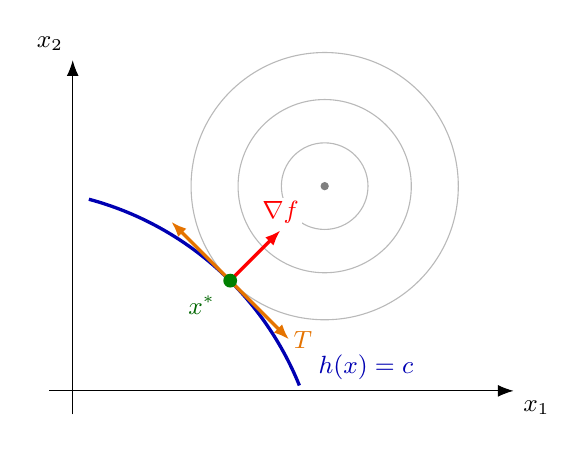
\begin{tikzpicture}[every node/.style={font=\small}, >={Latex[length=2mm]}, lab/.style={font=\small, fill=white, inner sep=1pt}]
	\draw[->] (-0.3,0) -- (5.6,0) node[below right] {$x_1$};
	\draw[->] (0,-0.3) -- (0,4.2) node[above left] {$x_2$};
	\foreach \r in {0.55,1.1,1.697} {\draw[gray!55] (3.2,2.6) circle (\r);}
	\fill[gray] (3.2,2.6) circle (1.5pt);
	\draw[blue!70!black, very thick] ([shift={(-0.83,-1.43)}]22:4) arc (22:75:4);
	\node[blue!70!black, anchor=west, font=\small] at (3.0,0.3) {$h(x)=c$};
	\draw[->, orange!90!black, very thick] (2.0,1.4) -- (2.75,0.65) node[right, lab] {$T$};
	\draw[->, orange!90!black, very thick] (2.0,1.4) -- (1.25,2.15);
	\draw[->, red, very thick] (2.0,1.4) -- (2.64,2.04) node[above, lab, yshift=1pt] {$\nabla f$};
	\fill[green!50!black] (2.0,1.4) circle (2.5pt);
	\node[green!40!black, anchor=north east, font=\small] at (1.93,1.33) {$x^\ast$};
\end{tikzpicture}
\end{document}
